\documentclass[conference,compsoc]{IEEEtran}

% *** CITATION PACKAGES ***
%
\ifCLASSOPTIONcompsoc
  % IEEE Computer Society needs nocompress option
  % requires cite.sty v4.0 or later (November 2003)
  \usepackage[nocompress]{cite}
\else
  % normal IEEE
  \usepackage{cite}
\fi
%\usepackage{graphicx}
%\usepackage{subcaption}
\usepackage{graphicx}
\graphicspath{ {images/} }
\usepackage{listings}
\usepackage[final]{pdfpages}
\usepackage{multicol}
\usepackage{dblfloatfix}
% correct bad hyphenation here
\hyphenation{op-tical net-works semi-conduc-tor}


\begin{document}
\begin{titlepage}
	\centering
	
\includegraphics[width=0.5\textwidth]{McGill_Logo}\par\vspace{1cm}
	{\scshape\LARGE McGill University \par}
	\vspace{1cm}
	{\scshape\Large ECSE 415 Project\par}
	\vspace{1.5cm}
	{\huge\bfseries Cat and Dog\par}
	\vspace{2cm}
	{\Large Jaeho Lee\par}
	{ 260633759\par} {\Large Raymond So \par} {260640297 \par}{Team name: You thought it was an original team name, \\but it was me, DIO!}
	\vfill
	submitting to\par
	Prof.~James \textsc{Clark}

	\vfill

% Bottom of the page
	{\large \today\par}
\end{titlepage}
%
% paper title
% Titles are generally capitalized except for words such as a, an, and, as,
% at, but, by, for, in, nor, of, on, or, the, to and up, which are usually
% not capitalized unless they are the first or last word of the title.
% Linebreaks \\ can be used within to get better formatting as desired.
% Do not put math or special symbols in the title.
\title{ECSE 415 Project\\ Cat and Dog}
\author{\IEEEauthorblockN{Jaeho Lee \IEEEauthorrefmark{1} and Raymond So \IEEEauthorrefmark{2}}
\IEEEauthorblockA{Department of Electrical Engineering, McGill University\\
\IEEEauthorrefmark{1}jaeho.lee2@mail.mcgill.ca, \IEEEauthorrefmark{2}raymond.su@mail.mcgill.ca}}

\maketitle



\IEEEpeerreviewmaketitle

\section{Introduction}
% no \IEEEPARstart
Most research for object classification was more focused on classifying images that are completely different (ex. horse and ship). In this project, we classify whether the image contains a picture of dog or cat. We were given 5906 images from [Cat and Dog paper]. We trained animal body detection and classification using 1500 images of cat and dog each. We used Haar features to detect the portion of the image containing the animal. Computation of the LBP histogram provides feature of the image for the classification. And then, we used  SVM to define whether the image contains dogs or cats.


\section{Problem Representation}
The goal of this project is to devise a machine learning algorithm to analyse images and classify them to their respective categories. The datasets for training and testing, which consist of 7384 images, were given from [kaggle website]. The ratio of dog and cat images in given dataset was 2:1. In order to fix training bias due to data inequality, we used external dataset from [cat face] which includes 4004 cat face, and 2271 cat ear images. \\

In order to tackle this problem, we built face detection and body detection in order to limit features to classify. Face detection is prior to be classified because it is easier and more accurate to classify if the detection system can detect face. If we include the entire body, there are numerous different data exists depends on gesture of the animal and photo inclusion of the animal (i.e photo includes only face, chest and up or the entire body). In [McGill Cat and Dog project paper], using classification based on face detection performed better than body detection. We used Haar feature detection from [Viola and Jones 2001] for both face detection and body detection\\

We used Local Binary Pattern (LBP) histogram from [LBP paper] to extract histogram data for classification. Consider we are using face detection, LBP histogram has advantage of face classification because LBP is fast and proven to perform well in classification based on face feature [LBP face detection]. After extract histogram data, Linear Support Vector Machine (LSVM) was used to classify whether the image includes cat or dog.

\section{Algorithm selection and implementation}
For object detection, we used Haar feature detection from [Viola and Jones 2001] for cascade trainer. Haar feature detection was chosen because we prior to use face detection and Haar performs fast and accurately [Viola Jones 2001]. We used pre-built OpenCV annotation program to select face and body region from the image. For body detection training, we used 3000 images from [kaggle website] dataset. For face detection training, we used 8000 images from [kaggle website] and [cat face] dataset. A vector file of image data was created before training in order to store annotated image data. After creating vector file, we trained the cascade to create a xml file. We used 14 stages for face detection and 17 stages for body detection. Before detect the face with test image, we use Gaussian filter to simplify features which increases detecting performance. Figure 1 addresses succeed and failed face detection example, figure 2 addresses succeed and failed body detection example.\\

After object detection, we use LBP from [LBP paper] and get histogram of face or body part. If the face detection program failed to detect face, body detection activates instead. We trained 2804 images for LBP from [kaggle website]. Single cell LBP was used because consider the face detection succeed, the image indicates the face of dog/cat is very small, therefore it would not be worth to use multiple cell LBP.\\

LSVM from sklearn library [sklearn library] was used to give linear line to separate dog and cat feature.

\begin{figure*}
	\begin{multicols}{4}
    		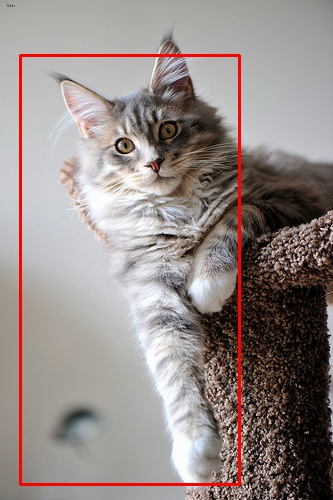
\includegraphics[height=1.35\linewidth]{naisubodi2.jpg}\par 
    		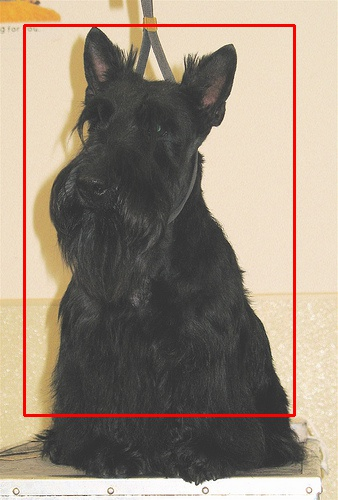
\includegraphics[height=1.35\linewidth]{good3.jpg}\par 
    		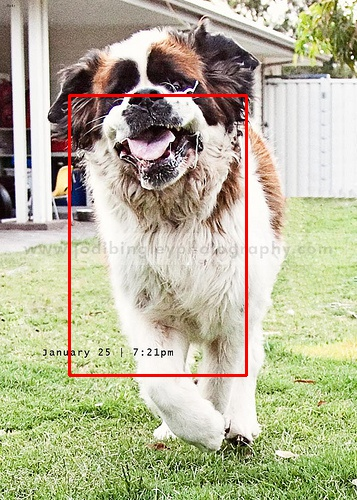
\includegraphics[height=1.35\linewidth]{terrible1.jpg}\par
    		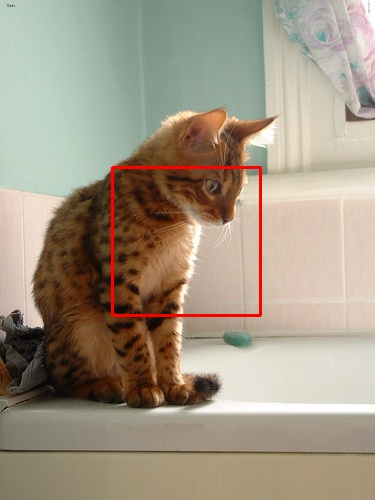
\includegraphics[height=1.35\linewidth]{terrible5.jpg}\par
	\end{multicols}
	\caption{Body detection result (left : succeed, right : failed)}
\end{figure*}
\begin{figure*}
	\begin{multicols}{4}
    		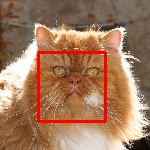
\includegraphics[height=1.35\linewidth]{goodFace2.jpg}\par 
    		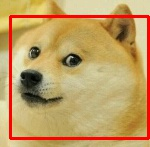
\includegraphics[height=1.35\linewidth]{dogeFace.jpg}\par 
    		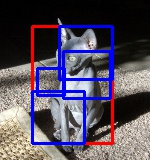
\includegraphics[height=1.35\linewidth]{smolrect.jpg}\par
    		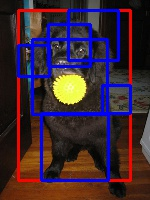
\includegraphics[height=1.35\linewidth]{smolrect2.jpg}\par
	\end{multicols}
	\caption{Face detection result (left : succeed, right : failed)}
\end{figure*}


\section{Testing}
The project is separated into two different section, object detection and classification.  This section describes how they were tested and the result of the project.
\subsection{Object Detection}
For both face and body detection, we trained the xml file with different number of stages, different distribution of face type, and different section of faces. With 4000 face images, cat detector performed best with 14~16 stages. Above 16 stages, the detector could not detect anything frequently. Below 14 stages, the detector includes wrong features and add unnecessary part which fails the purpose of face detection. Even with the optimized stages, we still could see the detector detects wrong features and adds unnecessary parts which is addressed in Figure 2. Right images include faces properly, however they also include other unnecessary parts which failed the face detection. Consider the image contains the face of animal in different angle, we distributed cat face photo before training. Out of 4000 cat face photos, we used 2500 front open eye, 800 front closed eye and 700 side view of the cat face which improved the performance in general. We also trained an additional training xml file consist of cat ear only. We used 2100 cat ear photo and ran the detection with cat face xml. However this did not improve the performance therefore we discarded it.\\

In case of body detection, it detects the entire or major parts of animal. Even in the failed cases, the detector succeed to detect the body of animal but did not include the entire body. However since part of animal is included we still could use classify program to decide whether the object is a cat or a dog. However the classification performance would drop because using entire body gives numerous characteristics which overwhelms LBP histogram classification [McGill Cat and Dog].
\subsection{Classification}
After classification, we obtained 66.6\% of accuracy which was below our expectation. The csv file is consist of mostly 1s which indicates the SVM is biased to dog. We suspect several different reasons which are briefly indicated in section 5.
\section{Discussion}


\begin{thebibliography}{1}

\bibitem{IEEEhowto:kopka}
K~. Smith, A~. Smith, \emph{Microelectronic circuits(Oxford series in electrical and computer engineering (Hardco)}, 7th~ed. New York, NY, United States: Oxford University Press, 2014.

\end{thebibliography}

\onecolumn

\end{document}


